\documentclass[11pt,a4paper]{article}

% ===============================================================================
% PREAMBLE & PACKAGES (Strict adherence to spec)
% ===============================================================================
\usepackage[margin=1.5cm, top=2cm, bottom=2cm]{geometry}
\usepackage{fontspec}
\setmainfont{Latin Modern Roman}
\setmonofont{Latin Modern Mono}
\usepackage{unicode-math}
\setmathfont{Latin Modern Math}
\usepackage{xcolor}
\usepackage{tikz}
\usetikzlibrary{shapes.geometric, arrows.meta, positioning, calc, fit, decorations.pathreplacing}
\usepackage[most]{tcolorbox}
\usepackage{tabularx, booktabs, array, multirow}
\usepackage{enumitem}
\usepackage{fancyhdr}
\usepackage{titlesec}
\usepackage{tocloft}
\usepackage{hyperref}

% ===============================================================================
% HYPHENATION & SPACING RULES
% ===============================================================================
\hyphenpenalty=10000
\exhyphenpenalty=10000
\sloppy

% ===============================================================================
% COLOR PALETTE (Strict adherence to spec)
% ===============================================================================
\definecolor{myred}{RGB}{196,30,58}       % section headings
\definecolor{mydark}{RGB}{30,30,50}       % body text
\definecolor{mygreen}{RGB}{14,120,80}     % definition boxes
\definecolor{myteal}{RGB}{0,130,140}      % formula boxes, diagrams, subsection headings
\definecolor{myamber}{RGB}{180,100,0}     % example boxes
\definecolor{mypurple}{RGB}{100,30,160}   % exam/viva boxes
\definecolor{myblue}{RGB}{25,90,170}      % hyperlinks/diagrams
\definecolor{mygray}{RGB}{246,247,249}    % tikzbox background
\definecolor{mgframe}{RGB}{180,185,200}   % tikzbox border
\definecolor{watermark}{RGB}{145,150,170} % footer watermark

\definecolor{hdrred}{RGB}{250,232,235}
\definecolor{hdrgreen}{RGB}{220,244,233}
\definecolor{hdrteal}{RGB}{220,242,244}
\definecolor{hdramber}{RGB}{253,242,215}
\definecolor{hdrpurple}{RGB}{238,228,255}
\definecolor{hdrblue}{RGB}{235,242,250}

% ===============================================================================
% TCOLORBOX STYLES (Standard MAKAUT Spec)
% ===============================================================================
\tcbset{
  tikzbox/.style={colback=mygray, colframe=mgframe, boxrule=0.6pt, arc=4pt,
    left=8pt, right=8pt, top=6pt, bottom=6pt,
    colbacktitle=mgframe, coltitle=mydark, fonttitle=\small\bfseries},
  defbox/.style={colback=hdrgreen, colframe=mygreen, boxrule=0.8pt, arc=4pt,
    left=9pt, right=9pt, top=6pt, bottom=6pt,
    colbacktitle=mygreen, coltitle=white, fonttitle=\small\bfseries},
  formulabox/.style={colback=hdrteal, colframe=myteal, boxrule=0.8pt, arc=4pt,
    left=9pt, right=9pt, top=7pt, bottom=7pt,
    colbacktitle=myteal, coltitle=white, fonttitle=\small\bfseries},
  examplebox/.style={colback=hdramber, colframe=myamber, boxrule=0.8pt, arc=4pt,
    left=9pt, right=9pt, top=6pt, bottom=6pt,
    colbacktitle=myamber, coltitle=white, fonttitle=\small\bfseries},
  masonbox/.style={colback=hdrpurple, colframe=mypurple, boxrule=0.8pt, arc=4pt,
    left=9pt, right=9pt, top=6pt, bottom=6pt,
    colbacktitle=mypurple, coltitle=white, fonttitle=\small\bfseries},
  exambox/.style={colback=hdrpurple, colframe=mypurple, boxrule=1pt, arc=5pt,
    left=10pt, right=10pt, top=8pt, bottom=8pt,
    colbacktitle=mypurple, coltitle=white, fonttitle=\bfseries,
    title after break={\textbf{Frequently Asked / Viva Questions (contd.)}}}
}
\tcbset{breakable}

% ===============================================================================
% TIKZ STYLES
% ===============================================================================
\tikzset{
  line/.style={draw=mydark, thick},
  arrow/.style={draw=mydark, -{Stealth[scale=1.2]}, thick},
  block/.style={draw=myteal, fill=hdrteal, rectangle, rounded corners=3pt, align=center, font=\small\bfseries, minimum height=0.8cm, text width=2.4cm}
}

% ===============================================================================
% TABLE COLUMNS & FORMATTING
% ===============================================================================
\newcolumntype{Y}{>{\raggedright\arraybackslash}X}
\newcolumntype{C}{>{\centering\arraybackslash}X}

% ===============================================================================
% SECTION FORMATTING
% ===============================================================================
\titleformat{\section}{\Large\bfseries\color{myred}}{\thesection}{1em}{}[\titlerule]
\titleformat{\subsection}{\large\bfseries\color{myteal}}{\thesubsection}{1em}{}
\titleformat{\subsubsection}{\bfseries\color{mydark}}{\thesubsubsection}{1em}{}

% ===============================================================================
% HEADER & FOOTER
% ===============================================================================
\pagestyle{fancy}
\fancyhf{}
\fancyhead[L]{\small\bfseries\color{mydark} OE-EC804C: Organizational Behavior}
\fancyhead[R]{\small\bfseries\color{myred} Module 2 Notes}
\fancyfoot[L]{\small\color{watermark} MAKAUT B.Tech ECE (2023--27)}
\fancyfoot[C]{\small\color{watermark} Page \thepage}
\fancyfoot[R]{\small\color{watermark} CGEC}
\renewcommand{\headrulewidth}{0.4pt}
\renewcommand{\footrulewidth}{0.4pt}

% ===============================================================================
% MACROS & COMMANDS
% ===============================================================================
\newcommand{\Q}[2]{\item \textbf{#1}\par #2 \vspace{4pt}}

\hypersetup{
  colorlinks=true,
  linkcolor=myteal,
  citecolor=mypurple,
  urlcolor=myblue,
  pdftitle={OE-EC804C Module 2 Notes},
  pdfauthor={Biraj Sarkar}
}

% ===============================================================================
% DOCUMENT STARTS HERE
% ===============================================================================
\begin{document}

% -------------------------------------------------------------------------------
% TITLE BLOCK
% -------------------------------------------------------------------------------
\begin{center}
  {\LARGE \bfseries \color{myred} OE-EC804C --- Organizational Behavior}\\[6pt]
  {\Large \bfseries \color{myteal} Module 2: Personality and Motivation}\\[4pt]
  {\small \color{mydark} Target Audience: MAKAUT B.Tech ECE 8th Semester $|$ Compiled by Biraj Sarkar (CGEC)}
\end{center}
\vspace{-6pt}
\hrule
\vspace{10pt}

% -------------------------------------------------------------------------------
% TABLE OF CONTENTS
% -------------------------------------------------------------------------------
\begin{tcolorbox}[tikzbox, title={Module Contents}]
\small
\tableofcontents
\end{tcolorbox}
\vspace{10pt}

% ===============================================================================
% 1. PERSONALITY AND DETERMINANTS
% ===============================================================================
\section{Personality: Concept and Determinants}

\textbf{Personality} represents the relatively stable set of psychological characteristics, behavioral patterns, and emotional tendencies that shape how an individual interacts with their environment.

\begin{tcolorbox}[defbox, title={Definition of Personality}]
  \textbf{Personality} is the dynamic organization within the individual of those psychophysical systems that determine their unique adjustments to their environment (Gordon Allport).
\end{tcolorbox}

\subsection{Determinants of Personality}
An individual's personality is shaped by four major determinants:

\begin{enumerate}[leftmargin=*, itemsep=4pt]
  \item \textbf{Heredity (Biological Factors):} Genetic traits inherited from parents (temperament, physical stature, reflexes, facial features). Twins studies show genetics accounts for nearly $50\%$ of personality variation.
  \item \textbf{Environmental Factors:} Socialization, family background, upbringing, social status, and educational experiences during early childhood.
  \item \textbf{Cultural Factors:} Cultural norms, values, beliefs, and societal expectations that dictate acceptable behavior.
  \item \textbf{Situational Factors:} Specific events, crises, or work situations that constrain or draw out specific personality dimensions.
\end{enumerate}

\subsection{Personality Development: Theories and Stages}
Personality development refers to the process by which an individual's unique behavioral patterns and psychological structures evolve over time:

\begin{enumerate}[leftmargin=*, itemsep=4pt]
  \item \textbf{Freud's Psychoanalytic Theory:} Personality consists of three interacting structural systems:
    \begin{itemize}[leftmargin=*, noitemsep]
      \item \textit{Id:} Unconscious, primitive drive operating on the pleasure principle.
      \item \textit{Ego:} Realistic, conscious executive operating on the reality principle.
      \item \textit{Superego:} Moral conscience representing societal norms and ethical ideals.
    \end{itemize}
  \item \textbf{Erikson's 8 Psychosocial Stages:} Personality evolves through 8 life stages characterized by specific psychosocial crises (e.g., Trust vs. Mistrust, Identity vs. Role Confusion, Industry vs. Inferiority).
  \item \textbf{Argyris' Immaturity-Maturity Continuum:} Chris Argyris proposed that individuals naturally progress along a continuum from infant \textbf{immaturity} (passive, dependent, short-term perspective) to adult \textbf{maturity} (active, independent, long-term perspective, self-awareness).
\end{enumerate}

% ===============================================================================
% 2. PERSONALITY THEORIES AND APPLICATIONS IN OB
% ===============================================================================
\section{Personality Theories and Applications in OB}

\subsection{The Big Five Personality Traits Model (OCEAN)}
The \textbf{Big Five Model} is the most widely validated framework for assessing personality traits in business settings:

\par\vspace{6pt}\noindent
\begingroup
\setlength{\tabcolsep}{5pt}%
\setlength{\extrarowheight}{3pt}%
\renewcommand{\arraystretch}{1.35}%
\begin{tabularx}{\linewidth}{|>{\raggedright\arraybackslash\bfseries}p{3.2cm}|Y|Y|}
\hline
\multicolumn{1}{|c|}{\textbf{Trait}} & \multicolumn{1}{c|}{\textbf{High Score Characteristics}} & \multicolumn{1}{c|}{\textbf{Organizational Impact}} \\
\hline
Openness to Experience & Creative, curious, imaginative, insightful, flexible. & Adapts quickly to organizational change \& innovation. \\
\hline
Conscientiousness & Organized, dependable, thorough, disciplined, goal-driven. & Single strongest predictor of overall job performance. \\
\hline
Extraversion & Sociable, assertive, energetic, outgoing, talkative. & Performs exceptionally in sales, leadership, \& networking. \\
\hline
Agreeableness & Cooperative, trusting, empathetic, warm, helpful. & Excels in teamwork, customer service, \& conflict resolution. \\
\hline
Emotional Stability (vs. Neuroticism) & Calm, self-confident, secure, stress-resilient. & High job satisfaction; low occupational burnout. \\
\hline
\end{tabularx}
\endgroup

\subsection{Major Personality Attributes Influencing OB}
\begin{itemize}[leftmargin=*, itemsep=4pt]
  \item \textbf{Locus of Control:} Belief about who controls destiny.
    \begin{itemize}[leftmargin=*, noitemsep]
      \item \textit{Internals:} Believe outcomes stem from their own effort. Higher job satisfaction \& performance.
      \item \textit{Externals:} Believe outcomes are driven by luck, fate, or external power. Higher stress.
    \end{itemize}
  \item \textbf{Machiavellianism (High-Mach):} Pragmatic, emotionally distant, and believes "the end justifies the means". Excels in high-stakes negotiations.
  \item \textbf{Type A vs. Type B Personality:}
    \begin{itemize}[leftmargin=*, noitemsep]
      \item \textit{Type A:} Impatient, competitive, time-conscious, aggressive. Prone to work stress.
      \item \textit{Type B:} Relaxed, patient, steady, non-competitive. Better long-term strategic thinkers.
    \end{itemize}
  \item \textbf{Self-Monitoring:} Ability to adjust behavior to external situational factors. High self-monitors are adept at political maneuvering.
\end{itemize}

% ===============================================================================
% 3. MOTIVATION CONCEPTS AND THEORIES
% ===============================================================================
\section{Motivation: Concepts and Theories}

\textbf{Motivation} is the psychological process that initiates, directs, and sustains goal-oriented human behavior.

\begin{tcolorbox}[defbox, title={Definition of Motivation}]
  \textbf{Motivation} is the willingness to exert high levels of effort toward organizational goals, conditioned by the effort's ability to satisfy some individual need (Robbins).
\end{tcolorbox}

\subsection{The Motivation-Behavior Process}

\begin{tcolorbox}[tikzbox, title={The 6-Stage Motivation-Behavior Process}]
\centering
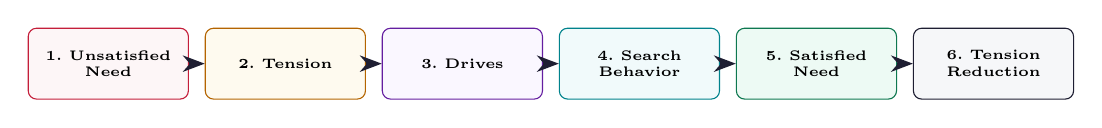
\begin{tikzpicture}[sblock/.style={rectangle, draw=mydark, fill=hdrteal!30, rounded corners=3pt, align=center, font=\tiny\bfseries, minimum height=0.9cm, text width=1.8cm}, node distance=0.2cm, auto]
  \node [sblock, fill=hdrred!40, draw=myred] (n) {1. Unsatisfied\\Need};
  \node [sblock, right=0.2cm of n, fill=hdramber!40, draw=myamber] (t) {2. Tension};
  \node [sblock, right=0.2cm of t, fill=hdrpurple!30, draw=mypurple] (d) {3. Drives};
  \node [sblock, right=0.2cm of d, fill=hdrteal!40, draw=myteal] (s) {4. Search\\Behavior};
  \node [sblock, right=0.2cm of s, fill=hdrgreen!50, draw=mygreen] (sat) {5. Satisfied\\Need};
  \node [sblock, right=0.2cm of sat, fill=mygray, draw=mydark] (r) {6. Tension\\Reduction};

  \draw [arrow] (n) -- (t);
  \draw [arrow] (t) -- (d);
  \draw [arrow] (d) -- (s);
  \draw [arrow] (s) -- (sat);
  \draw [arrow] (sat) -- (r);
\end{tikzpicture}
\end{tcolorbox}

\subsection{Maslow's Hierarchy of Needs Theory}
Abraham Maslow posited that human needs are arranged in a 5-level hierarchy. Individuals satisfy lower-order needs before progressing to higher-order needs:

\begin{tcolorbox}[tikzbox, title={Maslow's Hierarchy of Needs Pyramid}]
\centering
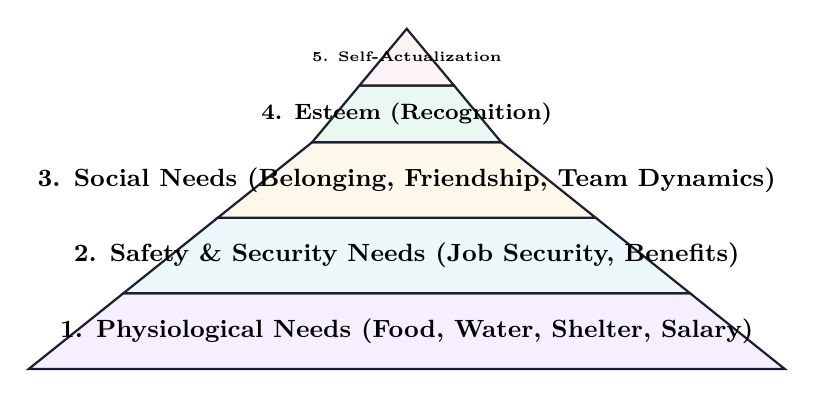
\begin{tikzpicture}[x=1.2cm, y=0.8cm]
  % Pyramid Slices
  \draw[line, fill=hdrpurple!60] (-4,0) -- (4,0) -- (3,1.2) -- (-3,1.2) -- cycle;
  \node at (0,0.6) {\small\textbf{1. Physiological Needs (Food, Water, Shelter, Salary)}};
  
  \draw[line, fill=hdrteal!50] (-3,1.2) -- (3,1.2) -- (2,2.4) -- (-2,2.4) -- cycle;
  \node at (0,1.8) {\small\textbf{2. Safety \& Security Needs (Job Security, Benefits)}};
  
  \draw[line, fill=hdramber!50] (-2,2.4) -- (2,2.4) -- (1,3.6) -- (-1,3.6) -- cycle;
  \node at (0,3.0) {\small\textbf{3. Social Needs (Belonging, Friendship, Team Dynamics)}};
  
  \draw[line, fill=hdrgreen!60] (-1,3.6) -- (1,3.6) -- (0.5,4.5) -- (-0.5,4.5) -- cycle;
  \node at (0,4.05) {\footnotesize\textbf{4. Esteem (Recognition)}};
  
  \draw[line, fill=hdrred!50] (-0.5,4.5) -- (0.5,4.5) -- (0,5.4) -- cycle;
  \node at (0,4.95) {\tiny\textbf{5. Self-Actualization}};
\end{tikzpicture}
\end{tcolorbox}

\subsection{Herzberg's Two-Factor (Hygiene-Motivator) Theory}
Frederick Herzberg proposed that job satisfaction and job dissatisfaction are driven by two independent sets of factors:

\par\vspace{6pt}\noindent
\begingroup
\setlength{\tabcolsep}{5pt}%
\setlength{\extrarowheight}{3pt}%
\renewcommand{\arraystretch}{1.35}%
\begin{tabularx}{\linewidth}{|>{\raggedright\arraybackslash\bfseries}p{3.5cm}|Y|Y|}
\hline
\multicolumn{1}{|c|}{\textbf{Dimension}} & \multicolumn{1}{c|}{\textbf{Hygiene Factors (Extrinsic)}} & \multicolumn{1}{c|}{\textbf{Motivators (Intrinsic)}} \\
\hline
Primary Impact & Prevents job dissatisfaction (does NOT create motivation). & Generates high job satisfaction \& intrinsic motivation. \\
\hline
Factors & Salary, company policies, working conditions, job security, supervision. & Achievement, recognition, responsibility, advancement, work itself. \\
\hline
Absence Result & Severe job dissatisfaction. & Neutral state (no satisfaction, but no dissatisfaction). \\
\hline
\end{tabularx}
\endgroup

\subsection{McGregor's Theory X and Theory Y}
Douglas McGregor formulated two contrasting views of human workforce motivation:

\par\vspace{6pt}\noindent
\begingroup
\setlength{\tabcolsep}{5pt}%
\setlength{\extrarowheight}{3pt}%
\renewcommand{\arraystretch}{1.35}%
\begin{tabularx}{\linewidth}{|>{\raggedright\arraybackslash\bfseries}p{3.5cm}|Y|Y|}
\hline
\multicolumn{1}{|c|}{\textbf{Assumption Area}} & \multicolumn{1}{c|}{\textbf{Theory X (Authoritarian View)}} & \multicolumn{1}{c|}{\textbf{Theory Y (Participative View)}} \\
\hline
Attitude Toward Work & Inherently dislike work and avoid it whenever possible. & View work as natural as play or rest. \\
\hline
Ambition \& Responsibility & Lack ambition, avoid responsibility, seek direction. & Exercise self-direction, seek responsibility. \\
\hline
Managerial Strategy & Strict control, coercion, punishment, close supervision. & Empowerment, delegation, participative decision-making. \\
\hline
Primary Motivator & Lower-order physiological \& safety needs. & Higher-order esteem \& self-actualization needs. \\
\hline
\end{tabularx}
\endgroup

% ===============================================================================
% 4. MOTIVATIONAL SYSTEMS AND INDIAN ORGANIZATIONAL CONTEXT
% ===============================================================================
\section{Elements of Sound Motivational System \& Indian Context}

\subsection{Elements of a Sound Motivational System}
A comprehensive managerial motivation strategy integrates financial and non-financial rewards:
\begin{itemize}[leftmargin=*, itemsep=4pt]
  \item \textbf{Fair \& Competitive Compensation:} Merit-based pay, profit sharing, and performance bonuses.
  \item \textbf{Job Enrichment:} Expanding job content vertically by giving greater autonomy, responsibility, and decision-making power.
  \item \textbf{Job Enlargement:} Expanding job content horizontally by adding a wider variety of similar tasks to eliminate monotony.
  \item \textbf{Employee Recognition Programs:} Awards, promotions, and public praise.
\end{itemize}

\subsection{Motivation in Indian Organizations}
Motivation strategies in Indian corporate environments account for cultural nuances (collectivism, respect for hierarchy, family orientation):
\begin{itemize}[leftmargin=*, itemsep=3pt]
  \item High value placed on \textbf{job security} and institutional stability.
  \item Paternalistic leadership style offering personal care alongside professional direction.
  \item Growing shift toward performance-linked incentives (PLI) and stock options (ESOPs) in tech startups and IT sectors.
\end{itemize}

% ===============================================================================
% QUICK REVISION PAGE
% ===============================================================================
\newpage
\begin{center}
  {\large\bfseries\color{myred} Quick Revision --- Module 2}\\[3pt]
  {\small\color{mydark} Personality and Motivation $|$ OE-EC804C}
\end{center}
\vspace{-4pt}
\hrule
\vspace{8pt}

\begin{tcolorbox}[formulabox, title={\textbf{Key Concepts and Metrics at a Glance}}]
\renewcommand{\arraystretch}{1.35}
\begin{tabularx}{\linewidth}{>{\raggedright\arraybackslash\bfseries}p{4.5cm} X}
Big Five OCEAN & Openness, Conscientiousness, Extraversion, Agreeableness, Neuroticism. \\[4pt]
Locus of Control & Internal (effort controls outcomes) vs. External (luck/fate controls outcomes). \\[4pt]
Maslow's Hierarchy & 5-stage needs pyramid: Physiological $\to$ Safety $\to$ Social $\to$ Esteem $\to$ Self-Actualization. \\[4pt]
Herzberg Two-Factor & Hygiene factors (salary/policy prevent dissatisfaction) vs. Motivators (responsibility/recognition build satisfaction). \\[4pt]
Theory X vs Theory Y & Lazy, coercive workforce view (Theory X) vs. Self-motivated, creative workforce view (Theory Y). \\
\end{tabularx}
\end{tcolorbox}

\begin{tcolorbox}[defbox, title={\textbf{One-Line Definitions for Exam Revision}}]
  \begin{itemize}[leftmargin=*, itemsep=2pt]
    \item \textbf{Conscientiousness:} Big Five trait reflecting organization, dependability, and goal discipline.
    \item \textbf{Machiavellianism:} Personality attribute characterized by emotional detachment and belief that ends justify means.
    \item \textbf{Job Enrichment:} Vertical expansion of job duties to increase employee autonomy and responsibility.
    \item \textbf{Hygiene Factors:} Extrinsic job factors whose presence prevents dissatisfaction but does not motivate.
  \end{itemize}
\end{tcolorbox}

\begin{tcolorbox}[exambox, title={\textbf{Frequently Asked / Viva Questions}}]
\begin{enumerate}[leftmargin=*, itemsep=4pt]
  \Q{Define Personality. What are its four main determinants?}{Personality is the dynamic organization of psychophysical systems determining an individual's unique adjustment to environment. Determinants: Heredity, Environment, Culture, and Situation.}
  
  \Q{List the Big Five personality traits (OCEAN). Which trait best predicts job performance?}{Openness, Conscientiousness, Extraversion, Agreeableness, and Neuroticism (Emotional Stability). Conscientiousness is the single best predictor of overall job performance.}
  
  \Q{Differentiate between Internal and External Locus of Control.}{Internals believe their own efforts determine success/failure; Externals believe outcomes are dictated by outside forces like luck, fate, or powerful people.}
  
  \Q{Compare Type A and Type B personalities.}{Type A individuals are impatient, competitive, aggressive, and time-driven; Type B individuals are relaxed, steady, patient, and less prone to stress.}
  
  \Q{Explain Maslow's Need Hierarchy Theory.}{Maslow proposed human needs follow a 5-tier pyramid: Physiological, Safety, Social, Esteem, and Self-Actualization. Individuals must fulfill lower-level needs before higher-level needs motivate them.}
  
  \Q{What are Hygiene Factors according to Herzberg? Give examples.}{Hygiene factors are extrinsic job elements (salary, company policy, working conditions) that prevent job dissatisfaction when present, but do not create positive motivation.}
  
  \Q{Contrast McGregor's Theory X and Theory Y.}{Theory X assumes workers are inherently lazy, dislike responsibility, and require coercion; Theory Y assumes workers are self-motivated, creative, and seek responsibility.}
  
  \Q{What is the difference between Job Enlargement and Job Enrichment?}{Job Enlargement expands work horizontally by adding similar tasks; Job Enrichment expands work vertically by adding autonomy, planning, and control.}
  
  \Q{Define Machiavellianism in an organizational context.}{It is a personality trait where an individual is pragmatic, maintains emotional distance, and manipulates situations believing the end justifies the means.}
  
  \Q{What factors influence employee motivation in Indian organizations?}{Job security, family-oriented benefits, respect for hierarchy, paternalistic leadership, and performance-linked incentives.}
\end{enumerate}
\end{tcolorbox}

\end{document}
